\newcommand{\vergelijkbaresystemen}{}
\label{sec:vergelijkbare-systemen}

Er bestaan al enkele oplossingen die functionaliteit bieden die vergelijkbaar is met die van de applicatie die wij gaan bouwen. Strava (Figuur~\ref{fig:strava}) en RunKeeper (Figuur~\ref{fig:runkeeper}) maken gebruik van GPS om onder andere hardlopers en wielrenners van realtime informatie te voorzien. MyLaps Practice (Figuur~\ref{fig:mylapspractice}) is een website waar je na je training je prestaties kan terugkijken. Er bestaat ook een iPhone App voor MyLaps Practice (Figuur~\ref{fig:mylapspractice-app}). Coach Watch (Figuur~\ref{fig:coachwatch}) is een iPad applicatie waarmee coaches hun teams kunnen volgen.

\begin{figure}[ht]
\centering
\subfigure[Strava]{
    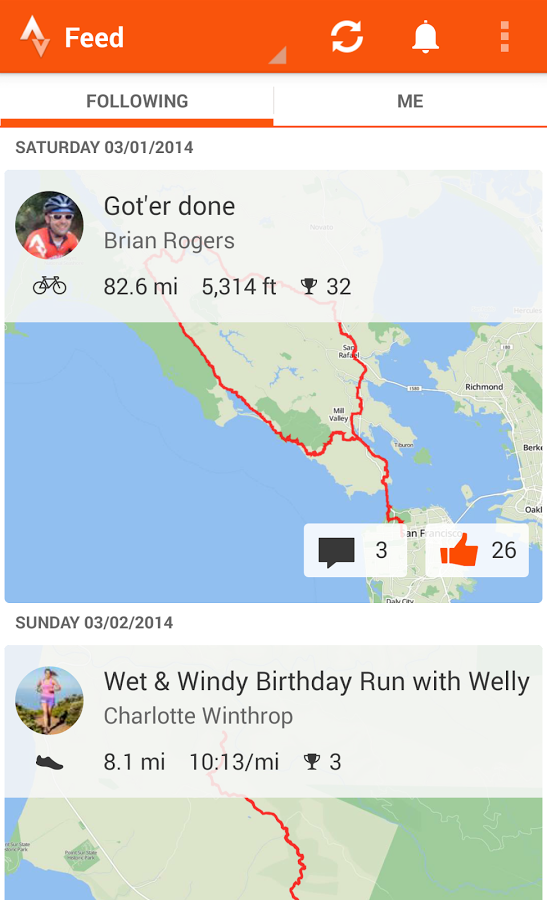
\includegraphics[height=5cm]{style/images/Strava}
    \label{fig:strava}
}
\subfigure[RunKeeper]{
    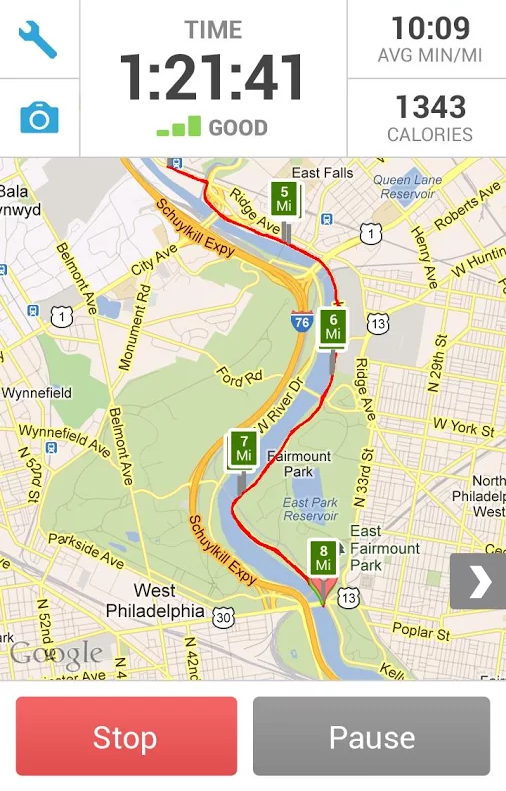
\includegraphics[height=5cm]{style/images/RunKeeper}
    \label{fig:runkeeper}
}
\subfigure[Coach Watch]{
    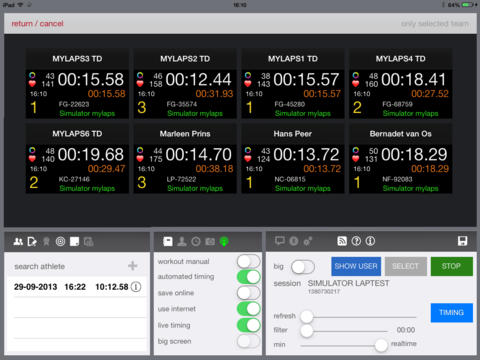
\includegraphics[height=5cm]{style/images/CoachWatch}
    \label{fig:coachwatch}
}

\subfigure[MyLaps Practice]{
    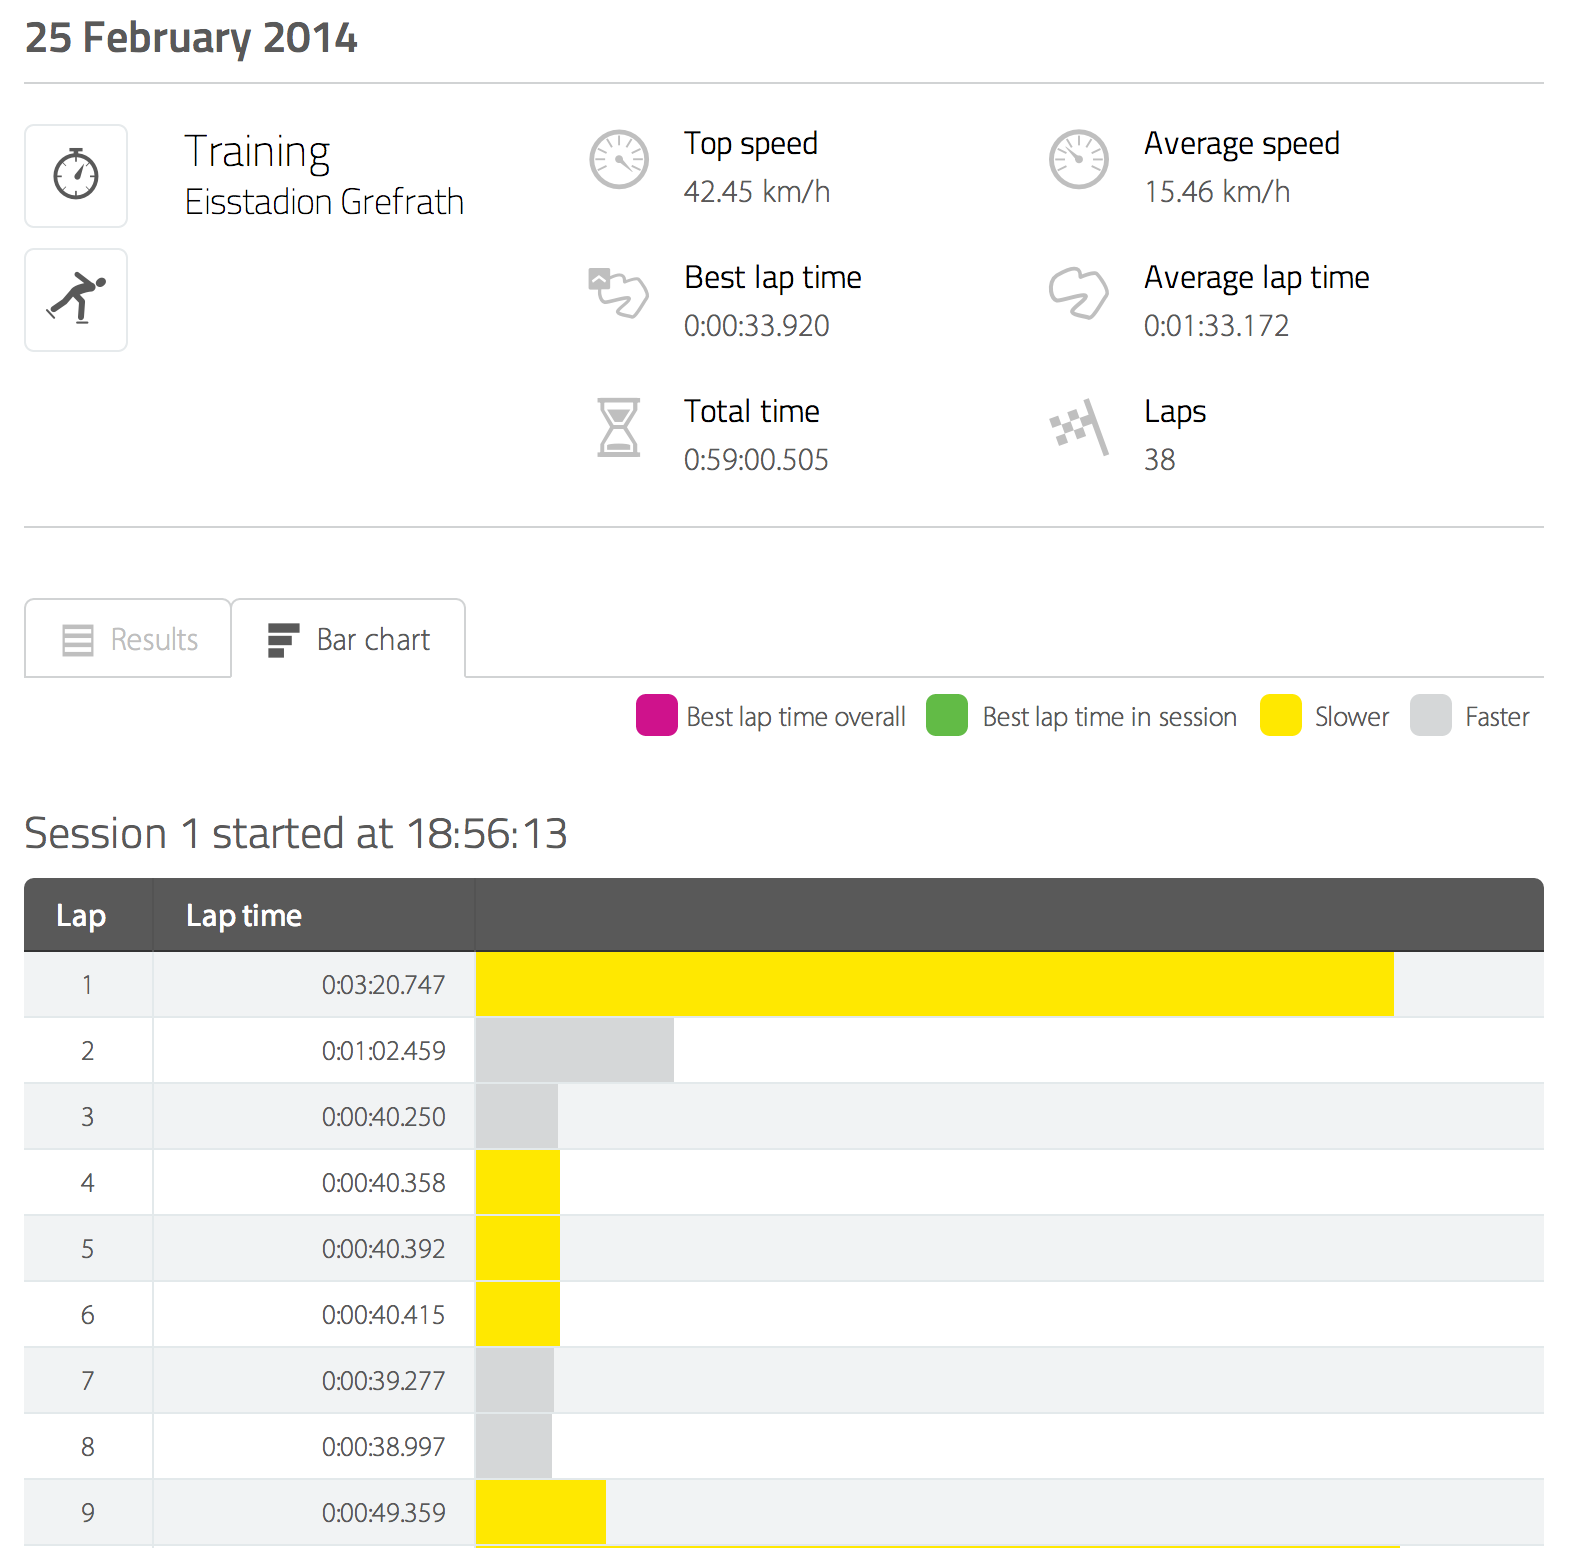
\includegraphics[height=7cm]{style/images/MyLapsPractice}
    \label{fig:mylapspractice}
}
\subfigure[MyLaps Practice App]{
    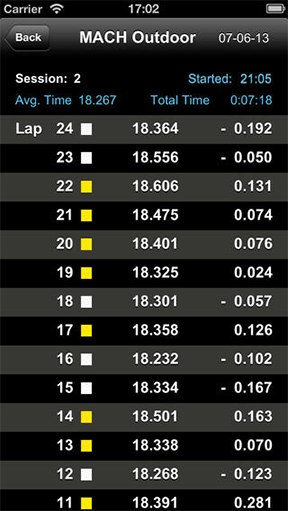
\includegraphics[height=7cm]{style/images/MyLapsPractice-App}
    \label{fig:mylapspractice-app}
}

\caption{Soortgelijke oplossingen}
\label{fig:soortgelijke-oplossingen}
\end{figure}

Strava en RunKeeper zijn voor baansporten, zoals bijvoorbeeld schaatsen, niet goed bruikbaar, aangezien GPS op de banen slecht presteert, waardoor de informatie niet nauwkeurig genoeg is. MyLaps Practice en Coach Watch maken wel gebruik van de detectielussen in de banen. De MyLaps Practice website kan alleen gebruikt worden voor het achteraf bekijken van sportprestaties en de App is vooral gericht op motorsporten. CoachWatch is een (vrij dure) applicatie die vooral gericht is op coaches en dus minder geschikt voor trainingen of amateursporters.

Emando ziet de mogelijkheid om een applicatie te bieden die gebruikmaakt van de detectielussen in de banen, live gegevens kan tonen op een smartphone en ook nog eens goedkoop of gratis is. Onze applicatie richt zich dus op het invullen van de stukken die missen in de bestaande oplossingen.